\chapter{今後の展望}
\label{chapter5}
最後に、本論文の研究に関して今後期待される展望とGroundBIRDの今後のアップデートの方針について述べる。
\section{大気揺らぎに由来するノイズのモデリング}
\label{atmos_model}
\ref{chapter4_3}章でスキャン軸上の検出器がより高い相関を持つこと、すなわちより同じ大気を観測するように改善されたことを見た。また、図\ref{compare_9011_11139}や図\ref{compare_9011_11679}にあるように、検出器間の相関の違いが\SI{10}{Hz}前後で顕著に出る結果を得た。この結果から大気放射ノイズは\SI{10}{Hz}前後の周波数で観測されていると考えられる。大気の揺らぎは非常に複雑であり、大気を何かしらのモデルによって単純化することが必要になる。本研究で、異なる検出器配置とその配置での相関の差を得られたため、両者の結果を矛盾なく説明する大気のモデル(大気の揺らぐ時間的、角度的スケール)を構築することができれば、GroundBIRDで観測する大気ノイズに対する系統的な理解を深めることが期待できる。ノイズの性質をより理解できれば、観測データから適切にノイズを差し引くことができ、CMBの偏光をより高精度に観測することにつながる。

ここでは、\cite{nishinomiya}の大気モデルを参考に、大気の相関に関する簡易的な考察を行う。大気のモデルとして、図\ref{atmos_layer}のように平面的な大気の層が重なっているものを考える。

\begin{figure}[htbp]
  \centering
  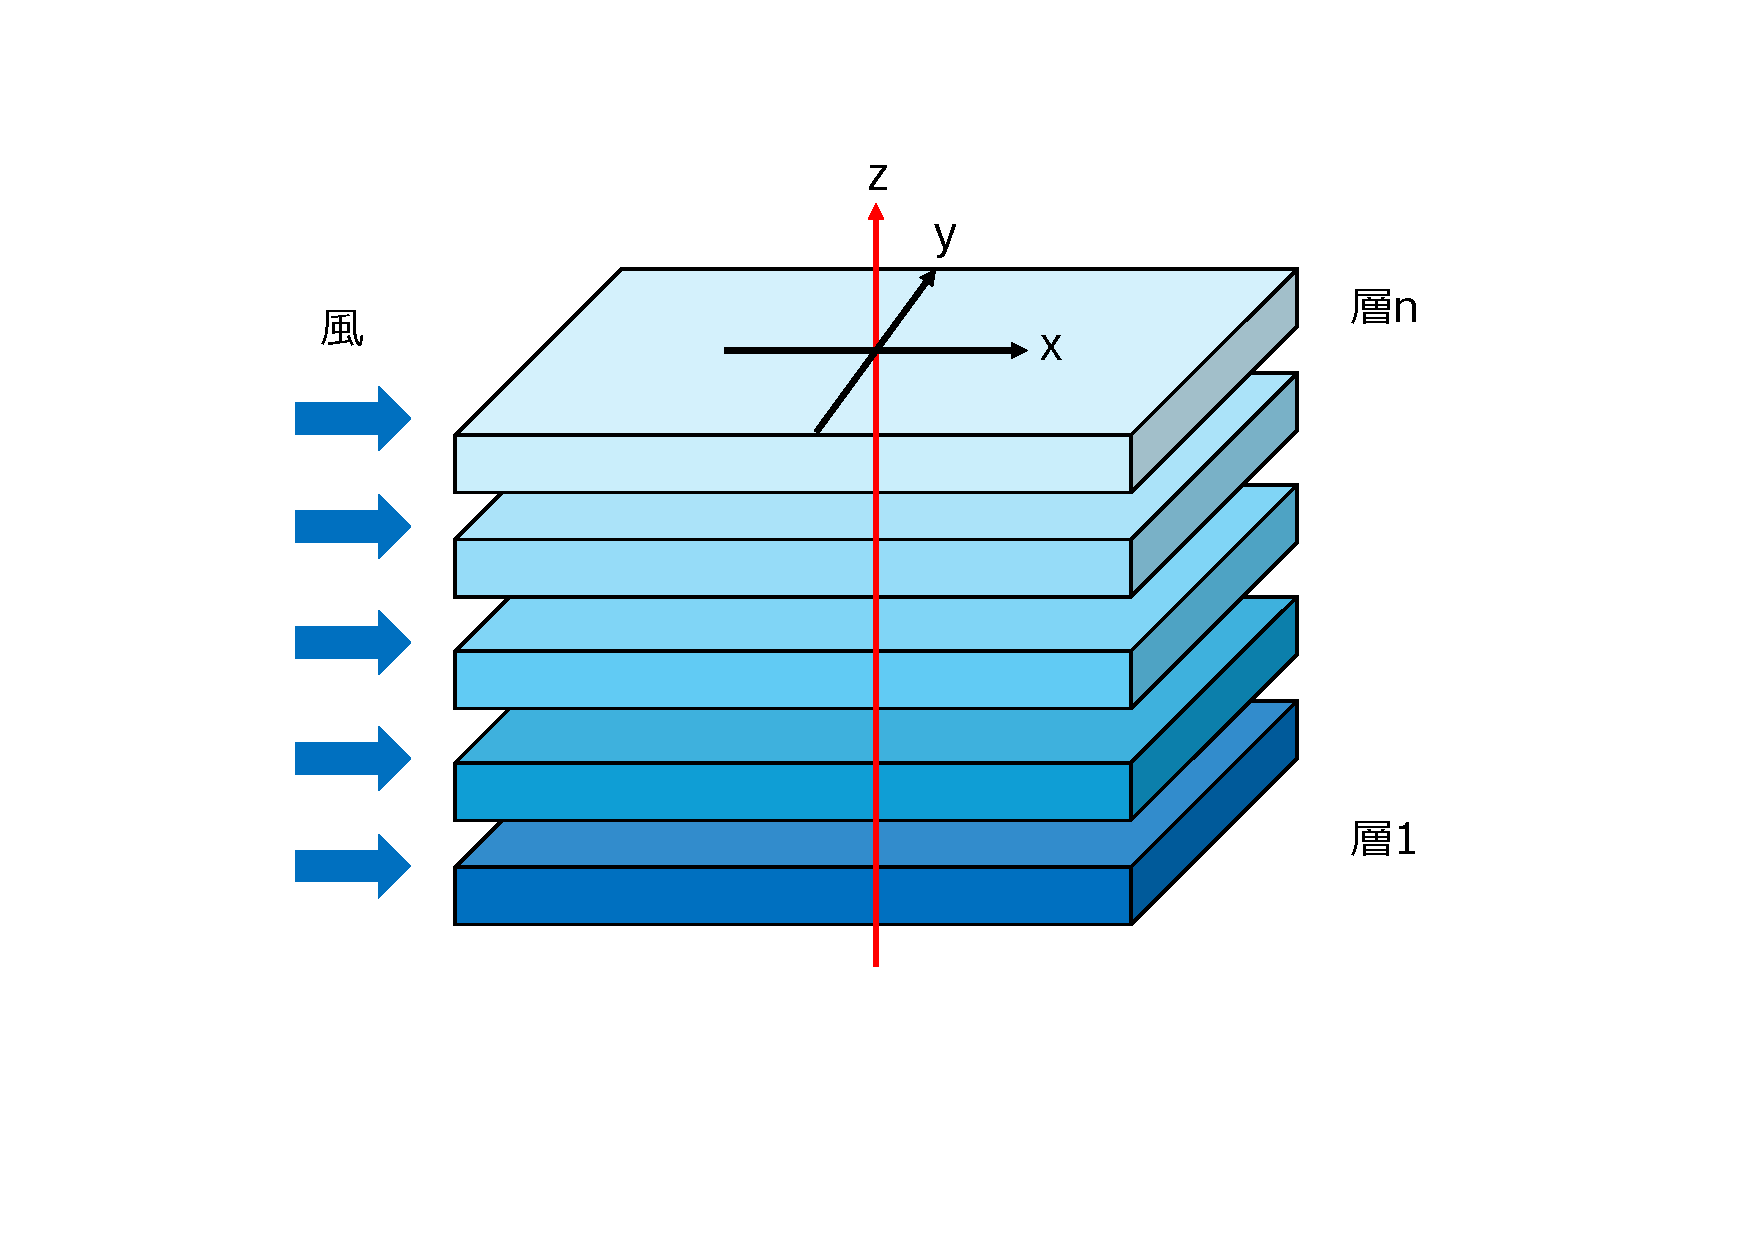
\includegraphics[width=0.7\columnwidth]{6_prospect/figs/atmos_layer.pdf}
  \caption{平面の層を用いた大気のモデル。望遠鏡の視線方向に$z$軸をとっている。また、全ての層は同じ風速の風を同じ方向に受けて動くと仮定している。}
  \label{atmos_layer}
\end{figure}
まず1層のみの場合で考える。層上の2つの検出器$i, j$があり、これらの座標の差を
\begin{equation}
  \Delta\bm{x} = (x_{i} -x_{j}, y_{i} - y_{j}) = (\Delta x, \Delta y)
\end{equation}
とする。この検出器間の相関を表す相関関数を
\begin{equation}
  R(\Delta\bm{x},\omega,z, v_{w}) = \frac{1}{2^{1/3}\Gamma(\frac{4}{3})}\mathrm{exp}\Bigl(i\frac{\omega}{v_{w}}\Delta x\Bigr)\Bigl(\frac{\omega}{v_{w}}|\Delta y|\Bigr)^{4/3}K_{4/3}\Bigl(\frac{\omega}{v_{w}}|\Delta y|\Bigr)
\end{equation}
と記述できる。ここで、$\omega$は周波数、$v_{w}$は風速、$K_{4/3}$は修正ベッセル関数を表す。

次に$n$層の場合を考える。全ての層同士は相関を持たないと仮定するため、多層であっても1層の場合でそれぞれ計算し、和を取ることで表せる。$i$番目の層までの距離を$z_{i}$とすると、$n$層での相関関数は
\begin{equation}
  R_{n}(\Delta\bm{\theta},\omega,v_{w}) = \frac{\displaystyle\sum_{i=1}^{n}w(z_{i})^{2}R(z_{i}\Delta\bm{\theta},\omega,z_{i},v_{w})}{\displaystyle\sum_{i=1}^{n}w(z_{i})^{2}}
\end{equation}
のように表せる。ここで、$\Delta\bm{\theta} = (\Delta x/z, \Delta y/z)$であり、$w(z)$は$z$の重み関数である。この相関関数は、風の方向に対して平行な向きを考えるとシンプルな表式になり、解析的に計算ができる。風に平行な向き、ここでは$x$方向のモデルを仮定して計算すると
\begin{align}
  R(\Delta\bm{\theta} = (\Delta\theta_{x}, 0), \omega, v_{w}) &= \frac{\int_{0}^{\infty}dz\mathrm{exp}\Bigl(-\frac{2z}{z_{0}}\Bigr)\mathrm{exp}\Bigl(i\frac{\omega}{v_{w}}z\Delta\theta_{x}\Bigr)}{\int_{0}^{\infty}dz\mathrm{exp}\Bigl(-\frac{2z}{z_{0}}\Bigr)} \\
  &= \frac{(\Gamma_{x}/2)^{2}}{(\Delta\theta_{x})^{2} + (\Gamma_{x}/2)^{2}} + i\frac{(\Gamma_{x}/2)\Delta\theta_{x}}{(\Delta\theta_{x})^{2} + (\Gamma_{x}/2)^{2}}
\end{align}
となる。$z_{0}$は重みのパラメータである。この時、相関関数の実部はローレンツ関数になり、対応するFWHMは
\begin{equation}
  \Gamma_{x} = \frac{4v_{w}}{z_{0}\omega}
\end{equation}
になる。この$\Gamma_{x}$~$[\mathrm{rad}]$を角度相関長として定義することができる。相関関数の実部の振る舞いを図\ref{correlation_real}に示す。
\begin{figure}[htbp]
  \centering
  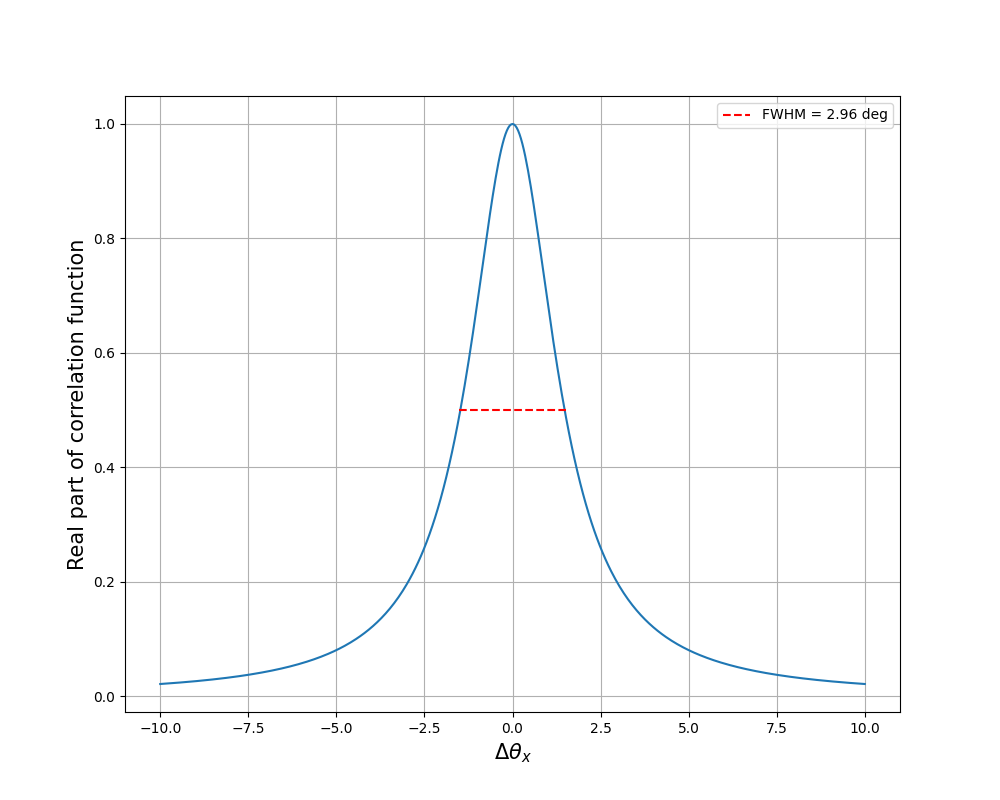
\includegraphics[width=0.8\columnwidth]{6_prospect/figs/correlation_real.png}
  \caption{風の向きに対して平行な向きでの相関関数の実部。半値全幅が角度相関長に対応する。横軸の$\Delta\theta_{x}$は$[\mathrm{deg}]$で表している。}
  \label{correlation_real}
\end{figure}
ここで、風速は観測所での典型的な値として、$v_{w}=\SI{20}{km/h}$とし、$z_{0}$と$\omega$は\cite{nishinomiya}の値を参照した。この設定での角度相関長は$\SI{2.96}{^{\circ}}$となり、この角度スケールで大気が相関を持つことになる。図\ref{6550_pos}や図\ref{10960_pos}で分かるように、同一スキャン軸上の検出器で見ている空の領域の仰角方向のずれはこの角度相関長より十分小さく、この指標では回転の前後での相関の差を十分には説明できない。
%この条件で望遠鏡を\SI{9}{RPM}でスキャンする時、スキャン角速度は$\SI{54}{\mathrm{deg/s}}$であるため、大気放射は$54/\Gamma_{x}\sim\SI{18}{Hz}$で観測される。これは図\ref{compare_9011_11139}や図\ref{compare_9011_11679}に見られる大気ノイズの周波数帯と一致する。この結果は大気をモデル化することで、観測データに現れる大気由来のノイズを説明できる可能性を示唆している。

本論文では最も単純なモデルで考察を行ったが、実際には風の方向に対して平行ではない状況もある他、風以外の条件を含める必要もあるため、大気ノイズの性質を説明するためにはより正確なモデルを構築する必要があると考えられる。今後の研究によって大気の詳細なモデルが作られ、ノイズを取り除く手法が確立されることが期待される。
\section{両偏波アンテナを搭載した焦点面検出器のアップデート}
GroundBIRDは将来計画として焦点面検出器を新たにアップデートすることを考えている。アップデートは主に次の2点からなる。
\begin{itemize}
  \item 両偏波を観測できるアンテナを搭載
  \item 多周波数帯を観測できるフィルターを搭載
\end{itemize}
現在の焦点面検出器は図\ref{full_array_mkid}にあるように、\SI{145}{GHz}アレイと\SI{220}{GHz}アレイから構成されている。また、感度のある偏光方向はそれぞれのMKIDで1方向である。そのため、1つのピクセルは1つの周波数帯と1つの偏光方向を観測できる性能に留まっている。それに伴って、偏光を観測するには異なるピクセルとの差分を取る必要が生じる。\ref{chapter4_1}章で見たように差分をとり、ノイズを取り除くことで偏光を観測できるが、スキャンによるtiming offsetを考慮する必要があり、TODの処理が複雑になってしまう。この問題を解決するために、1つのピクセルで2偏波を観測できるような両偏波アンテナを搭載したMKIDにアップデートする。これにより、同一ピクセルで同じ大気を同時に観測できるため、観測性能が大きく向上する上、時間差を考慮する必要もない。

また、複数の周波数帯をカバーできるフィルターを搭載することで1つの検出器で\SI{145}{GHz}帯と\SI{220}{GHz}帯の両方を観測できるようになり、有効的な検出器数を大きく増やすことができる。これによって統計量を稼ぐことが可能となる。現在は新しい検出器アレイのデザインが考案されており(図\ref{new_kid})、製作に向けて準備が進んでいる。
\begin{figure}[htbp]
  \centering
  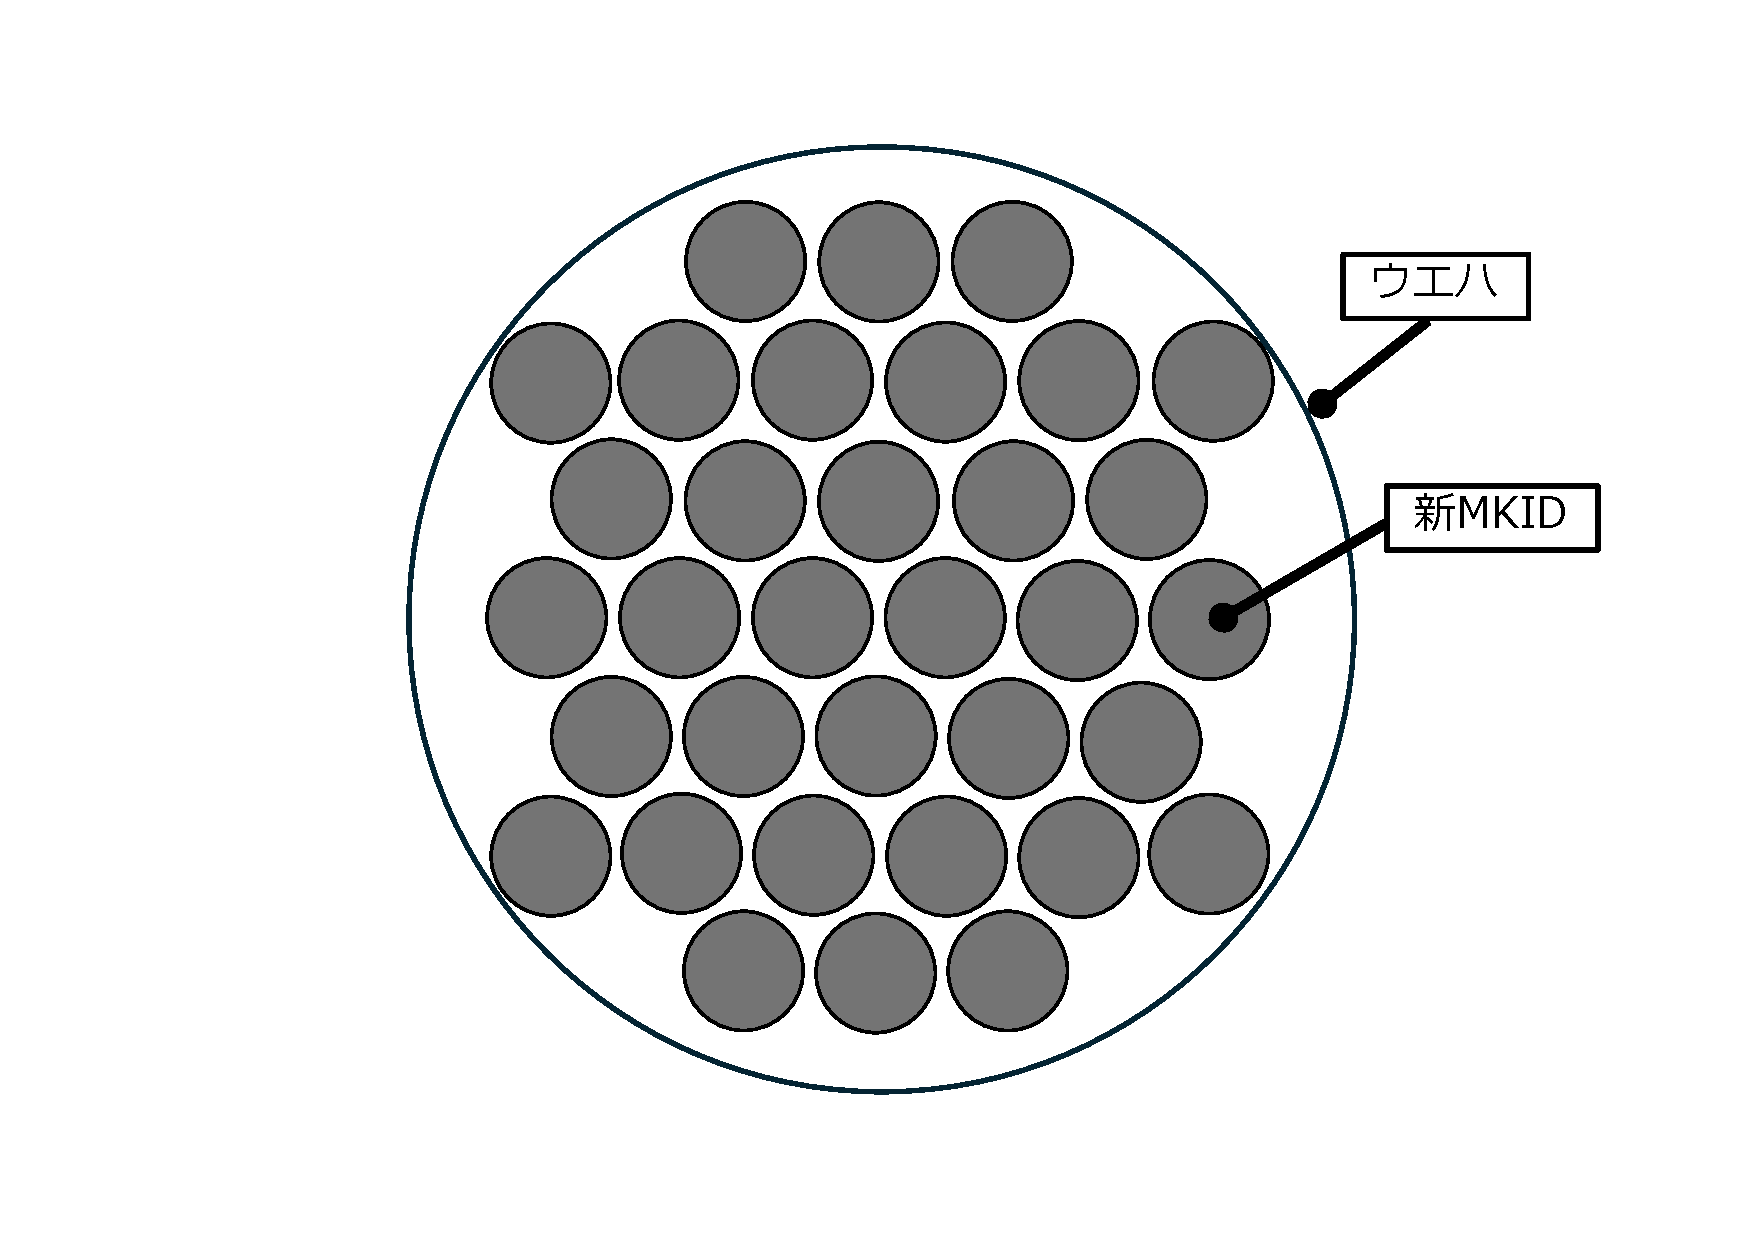
\includegraphics[width=0.75\columnwidth]{6_prospect/figs/new_kid.pdf}
  \caption{現在考案中の検出器アレイの模式図。実際は焦点面に160ピクセルの検出器を並べるようなデザインとなっている。両方の周波数帯を観測できるため、アレイを区切って役割を分担させる必要がない。}
  \label{new_kid}
\end{figure}

焦点面検出器をより高機能化、多機能化する上で、現在の検出器での観測から得た知見を引き継ぐことが重要である。大気の観測やモデリングを通して、大気ノイズやその揺らぎの性質を明らかにし、その情報を新しい検出器にも適用することで、精度の良いCMB偏光観測につながる。本研究によって将来のアップデートに向けた長期観測が進み、多くの理解を深めた上で新検出器に引き継ぐことが期待される。
%\section{人がいない件}

%人が足りていないのでもっと人を雇うべきだと思う。

%\section{LiteBIRDの未来}

%LiteBIRDの未来はない by Osamu
